\section{Valutazione dell'intervento}
Vedremo in questa sezione i dettagli che hanno caratterizzato la fase di user teting. 
Nello specifico vedremo il protocollo di User Testing utilizzato, i
risultati ottenute dalle valutazioni, la loro analisi e le migliorie
apportate all'interfaccia di CookApp a seguito dello studio dei
risultati.

%\subsection{Ispezione}

\subsection{User Testing}

Come per la valutazione dei sistemi già esistenti, ci siamo affidati
alla tipoligia di test Discount usability teting.

\subsubsection*{Elenco dei task da testare}
Per questa fase di sviluppo, abbiamo scelto un sottoinsieme dei task già definiti in precedenza
nell'analisi della fattibilità (\ref{task}) da utilizzare nello user
testing. Abbiamo prestato particolare attenzione verso i task
considerati più importanti e più critici. Inoltre alcuni di essi non
sarebbero testabili senza uno sviluppo completo dell'applicazione.

\begin{enumerate}
\item Impostare il livello di preparazione culinaria
\item Accedere alla documentazione/help dell'applicazione

\item Ricerca di una ricetta per nome.
\item Ricerca di una ricetta per ingredienti.

\item Ricerca di una ricetta sfogliando le categorie.

\item Filtro di una ricerca in base agli ingredienti.
\item Filtro di una ricerca in base alle intolleranze/allergie/diete.

\item Individuare la difficoltà di preparazione e il costo di una ricetta.
\item Individuare gli ingredienti necessari alla preparazione di una ricetta.
\item Distinguere le varie fasi di una preparazione della ricetta.
\item Distinguere la vista passo-passo della preparazione dalla visione complessiva della ricetta.
\item Visionare un video di presentazione della ricetta
\item Condividere una ricetta sui social network.
\item Creare un menù completo selezionando una lista di ricette.
\item Aggiungere/Rimuovere una ricetta al menù già creato.
\item Cercare un menù consigliato da CookApp.

\item Inserire una nuova ricetta nel database dell'applicazione.
\item Interagire con la community rispondendo a problemi degli utenti.
\item Chiedere consiglio alla community creando un nuovo topic.
\item Chiedere aiuto "live" alla community riguardo un particolare
passaggio della ricetta oppure riguardo agli ingredienti.

\item Salvare/Rimuovere una ricetta nei preferiti.
\item Salvare/Rimuovere un menù nei preferiti.

\item Accedere alla lista della spesa.
\item Inserire/Rimuovere gli ingredienti di una ricetta nella lista della spesa.
\item Inserire/Rimuovere gli ingredienti di un menù nella lista della spesa.

\item Votare e commentare le ricette ed i menu.

\item Visualizzare il progresso della preparazione del menù e della singola ricetta

\item Trova i punti vendita degli ingredienti della lista della spesa.
\item Aggiungere/confermare una voce nella lista della spesa.
\item Interagire con la mappa del percorso mediante lo smartwatch per strada e nel punto vendita.
\item Aggiungere/confermare una voce nella lista della spesa con lo smartwatch.
\end{enumerate}

\subsubsection*{Sistemi utilizzati}
Sono stati utilizzati tre sistemi:
\begin{itemize}
\item Un portatile HP Omen Touchscreen - Windows 10
\item Microsoft Surface Pro 3
\item un prototipo cartaceo di smartwatch.
\end{itemize}
Tramite i primi due sono state testati tutte i task, mentre con il
prototipo di smartwatch sono stati testati i task che riguardano la
lista della spesa e l'interazione con la mappa dei punti vendita e la
navigazione interna ad un locale.
\subsubsection*{Numero di test e numero di utenti}
Cinque test e cinque utenti.
\subsubsection*{Metodologia di testing}
Come per la valutazione di sistemi esistenti è stato preferito il metodo
\emph{Thinking Aloud}.
\subsubsection*{Analisi dei risultati}
Vedremo task per task la difficoltà attesa media, la difficoltà
 riscontrata media, gli eventuali errori commessi, la percentuale di
completamento del task ed eventuali note del tester.
\begin{itemize}

\item 
\textbf{Task 1: impostare il livello di preparazione culinaria}\\
\textbf{Difficoltà attesa (media):} 2/5\\
\textbf{Difficoltà riscontrata (media):} 1/5\\
\textbf{Task Completato:} 100\%\\
\textbf{Note:} Solo un utente non ha individuato immediatamente il
profilo, ma dopo averlo fatto ha portato a termine il task come tutti
gli altri.\\

\item
\textbf{Task 2: accedere alla documentazione/help dell'applicazione}\\
\textbf{Difficoltà attesa (media):} 1/5\\
\textbf{Difficoltà riscontrata (media):} 1/5\\
\textbf{Task Completato:} 100\%\\

\item
\textbf{Task 3: ricerca di una ricetta per nome}\\
\textbf{Difficoltà attesa (media):} 1/5\\
\textbf{Difficoltà riscontrata (media):} 1/5\\
\textbf{Task Completato:} 100\%\\\\

\item
\textbf{Task 4: ricerca di una ricetta per ingrediente}\\
\textbf{Difficoltà attesa (media):} 1/5\\
\textbf{Difficoltà riscontrata (media):} 1/5\\
\textbf{Task Completato:} 100\%\\\\

\item
\textbf{Task 5: ricerca di una ricetta sfogliando le categorie}\\
\textbf{Difficoltà attesa (media):} 1/5\\
\textbf{Difficoltà riscontrata (media):} 1/5\\
\textbf{Task Completato:} 100\%\\\\

\item
\textbf{Task 6: filtro di una ricerca in base agli ingredienti}\\
\textbf{Difficoltà attesa (media):} 2/5\\
\textbf{Difficoltà riscontrata (media):} 2/5\\
\textbf{Task Completato:} 100\%\\\\
\textbf{Note:} Un utente ha impiegato qualche secondo per capire che i
filtri di default erano tutti selezionati.

\item
\textbf{Task 7: filtro di una ricerca in base alle intolleranze/allergie/diete}\\
\textbf{Difficoltà attesa (media):} 3/5\\
\textbf{Difficoltà riscontrata (media):} 2/5\\
\textbf{Task Completato:} 100\%\\

\item
\textbf{Task 8: individuare la difficoltà di preparazione e il costo di una ricetta}\\
\textbf{Difficoltà attesa (media):} 1/5\\
\textbf{Difficoltà riscontrata (media):} 1/5\\
\textbf{Task Completato:} 100\%\\
\textbf{Note:} due utenti hanno avuto leggere difficoltà a distinguere
il significato della differenza di colore tra i cappelli che indicano la
difficoltà di preparazione e il colore degli euri che indicano il
costo.

\item
\textbf{Task 9: individuare gli ingredienti necessari alla preparazione
di una ricetta}\\
\textbf{Difficoltà attesa (media):} 1/5\\
\textbf{Difficoltà riscontrata (media):} 1/5\\
\textbf{Task Completato:} 100\%\\

\item
\textbf{Task 10: distinguere le varie fasi di una preparazione della
ricetta.}\\
\textbf{Difficoltà attesa (media):} 2/5\\
\textbf{Difficoltà riscontrata (media):} 1/5\\
\textbf{Task Completato:} 100\%\\

\item
\textbf{Task 11: distinguere la vista passo-passo dalla visione
complessiva della ricetta}\\
\textbf{Difficoltà attesa (media):} 2/5\\
\textbf{Difficoltà riscontrata (media):} 1/5\\
\textbf{Task Completato:} 100\%\\

\item
\textbf{Task 12: visionare un video di presentazione della ricetta}\\
\textbf{Difficoltà attesa (media):} 1/5\\
\textbf{Difficoltà riscontrata (media):} 1/5\\
\textbf{Task Completato:} 100\%\\

\item
\textbf{Task 13: condividere una ricetta sui social network}\\
\textbf{Difficoltà attesa (media):} 2/5\\
\textbf{Difficoltà riscontrata (media):} 1/5\\
\textbf{Task Completato:} 100\%\\
\textbf{Note}: solo un utente, non abile con i social network, ha
impiegato un po' di tempo per capire la funzionalità del task.\\

\item
\textbf{Task 14: creare un menù completo selezionando una lista di
ricette.}\\
\textbf{Difficoltà attesa (media):} 3/5\\
\textbf{Difficoltà riscontrata (media):} 2/5\\
\textbf{Task Completato:} 100\%\\

\item
\textbf{Task 15: aggiungere/rimuovere una ricetta al menù già creato.}\\
\textbf{Difficoltà attesa (media):} 2/5\\
\textbf{Difficoltà riscontrata (media):} 2/5\\
\textbf{Task Completato:} 100\%\\
\textbf{Note:} qualche utente ha avuto difficoltà nell'individuare la
ricetta aggiunta ad menù all'interno della sezione ``I miei menù''. Il
task è comunque stato completato da tutti gli utenti.\\

\item
\textbf{Task 16: cercare un menù consigliato da CookApp}\\
\textbf{Difficoltà attesa (media):} 1/5\\
\textbf{Difficoltà riscontrata (media):} 1/5\\
\textbf{Task Completato:} 100\%\\

\item
\textbf{Task 17: inserire una nuova ricetta nel database
dell'applicazione}\\
\textbf{Difficoltà attesa (media):} 2/5\\
\textbf{Difficoltà riscontrata (media):} 2/5\\
\textbf{Task Completato:} 100\%\\
\textbf{Errori commessi:} un utente ha chiuso il form della creazione
della ricetta prima di confermare, ma ha comunque completato il tast
grazie ad un avviso dell'applicazione.\\

\item
\textbf{Task 18: interagire con la community rispondendo a problemi
degli utenti}\\
\textbf{Difficoltà attesa (media):} 2/5\\
\textbf{Difficoltà riscontrata (media):} 2/5\\
\textbf{Task Completato:} 100\%\\
\textbf{Note}: un utente ha impiegato un po' di tempo per comprendere la
differenza tra richiesta della community e un aiuto LIVE per una fase di
preparazione.

\item
\textbf{Task 19: chiedere consiglio alla community creando un nuovo
topic}\\
\textbf{Difficoltà attesa (media):} 1/5\\
\textbf{Difficoltà riscontrata (media):} 1/5\\
\textbf{Task Completato:} 100\%\\

\item
\textbf{Task 20: chiedere aiuto ``live'' alla cummunity riguardo un
particolare passaggio della ricetta oppure riguardo agli ingredienti}\\
\textbf{Difficoltà attesa (media):} 2/5\\
\textbf{Difficoltà riscontrata (media):} 3/5\\
\textbf{Task Completato:} 60\%\\
\textbf{Errori}: due utenti non hanno individuato il pulsante di
richiesta d'aiuto. A causa di ciò non sono riusciti a completare il
task.

\item
\textbf{Task 21: salvare/rimuovere una ricetta dai preferiti}\\
\textbf{Difficoltà attesa (media):} 1/5\\
\textbf{Difficoltà riscontrata (media):} 1/5\\
\textbf{Task Completato:} 100\%\\
\textbf{Note:} solo due utente hanno individuato la scorciatoia per
esperti utilizzabile per la rimozione di una ricetta dai preferiti.
Tutto hanno comunque completato il task nella modalità standard.

\item
\textbf{Task 22: salvare/rimuovere un menù nei preferiti}\\
\textbf{Difficoltà attesa (media):} 1/5\\
\textbf{Difficoltà riscontrata (media):} 2/5\\
\textbf{Task Completato:} 100\%\\
\textbf{Errori:} un utente ha cercato inizialmente un opzione per
rimuovere un menù dalla sezione ``I miei menù'' confondendola con i
preferiti. Non trovandola ha
poi selezionato il menù e trovato il pulsante per rimuoverlo dai
preferiti.

\item
\textbf{Task 23: accedere alla lista della spesa}\\
\textbf{Difficoltà attesa (media):} 1/5\\
\textbf{Difficoltà riscontrata (media):} 1/5\\
\textbf{Task Completato:} 100\%\\

\item
\textbf{Task 24: inserire/rimuovere gl ingredienti di una ricetta nella
lista della spesa}\\
\textbf{Difficoltà attesa (media):} 1/5\\
\textbf{Difficoltà riscontrata (media):} 2/5\\
\textbf{Task Completato:} 100\%\\
\textbf{Note}: qualche utente ha avuto confusione nel capire se fossero
stati aggiunti tutti o solo alcuni gli ingredienti della ricetta alla
lista della spesa.

\item
\textbf{Task 25: inserire/rimuovere gli ingredienti di un menù nella
lista della spesa.}\\
\textbf{Difficoltà attesa (media):} 1/5\\
\textbf{Difficoltà riscontrata (media):} 2/5\\
\textbf{Task Completato:} 100\%\\
\textbf{Note}: qualche utente ha avuto confusione nel capire se fossero
stati aggiunti tutti o solo alcuni gli ingredienti del menù alla lista
della spesa.

\item
\textbf{Task 26: votare e commentare le ricette ed i menù}\\
\textbf{Difficoltà attesa (media):} 2/5\\
\textbf{Difficoltà riscontrata (media):} 1/5\\
\textbf{Task Completato:} 100\%\\

\item
\textbf{Task 27: visualizzare il progresso della preparazione del menù e
della singola ricetta}\\
\textbf{Difficoltà attesa (media):} 3/5\\
\textbf{Difficoltà riscontrata (media):} 1/5\\
\textbf{Task Completato:} 100\%\\
\textbf{Note}: tutti gli utenti hanno apprezzato l'utilità e la facilità
di comprensione di questa funzionalità. Un utente avrebbe preferito
anche una modalità esperta per parallelizzare le fasi di preprarazione.

\item
\textbf{Task 28: trova i punti vendita degli ingredienti della lista
della spesa}\\
\textbf{Difficoltà attesa (media):} 3/5\\
\textbf{Difficoltà riscontrata (media):} 1/5\\
\textbf{Task Completato:} 100\%\\

\item
\textbf{Task 29: aggiungere/confermare una voce nella lista della spesa}
\textbf{Difficoltà attesa (media):} 3/5\\
\textbf{Difficoltà riscontrata (media):} 2/5\\
\textbf{Task Completato:} 100\%\\
\textbf{Errori}: due utenti hanno confuso il tasto annulla con il tasto per
l'eliminazione di un ingrediente. Hanno comunque portato a termine il task
avendo subito appreso la funzionalità del pulsante dopo l'errore.

\item
\textbf{Task 30: Interagire con la mappa del percorso mediante lo
smartwatch per strada e nel punto vendita}\\
\textbf{Difficoltà attesa (media):} 4/5\\
\textbf{Difficoltà riscontrata (media):} 1/5\\
\textbf{Task Completato:} 100\%\\
\textbf{Note}: quasi tutti gli utenti hanno dichiarato di aver presupposto un alto livello
di difficoltà in quanto non credevano fosse possibile conoscere la
posizione degli ingredienti all'interno di un punto vendita. Tutti gli
utenti hanno trovato l'interfaccia per smartwatch molto intuitiva

\item
\textbf{Task 31: aggiungere/confermare una voce nella lista della spesa con
lo smartwatch}\\
\textbf{Difficoltà attesa (media):} 3/5\\
\textbf{Difficoltà riscontrata (media):} 1/5\\
\textbf{Task Completato:} 100\%\\
\end{itemize}

Sono stati individuati 4 errori cosmetici, 3 errori minori, 2 errori
gravi ed 1 catastrofico:

\begin{itemize}
	\item \textbf{Errori cosmetici}
		\begin{itemize}
			\item \textbf{Task 6: filtro di una ricerca in base agli ingredienti}\\
				\textbf{Problema:} un utente ha impiegato qualche secondo per capire che i
				filtri di default erano tutti selezionati.\\
				\textbf{Impatto:} 1\\
				\textbf{Frequenza:} 1\\

			\item \textbf{Task 8: individuare la difficoltà di preparazione e il costo di una ricetta}\\
				\textbf{Problema:} due utenti hanno avuto leggere difficoltà a distinguere
				il significato della differenza di colore tra i cappelli che indicano la
				difficoltà di preparazione e il colore degli euri che indicano il
				costo.\\
				\textbf{Suggerimento:} usare lo stesso colore per i due tipi di icona.\\
				\textbf{Impatto:} 1\\
				\textbf{Frequenza:} 2\\

			\item \textbf{Task 17: inserire una nuova ricetta nel database
				dell'applicazione}\\
				\textbf{Problema:} un utente ha chiuso il form della creazione
				della ricetta prima di confermare, ma ha comunque completato il tast
				grazie ad un avviso dell'applicazione.\\
				\textbf{Impatto:} 2 \\
				\textbf{Frequenza:} 1\\
			
			\item \textbf{Task 21: salvare/rimuovere una ricetta dai preferiti}\\
				\textbf{Problema:} solo due utenti hanno individuato la scorciatoia per
				esperti utilizzabile per la rimozione di una ricetta dai preferiti.
				Tutto hanno comunque completato il task nella modalità standard.\\
				\textbf{Suggerimento:} aggiungere un invito
				nell'interfaccia che permetta di capire come abilitare la scorciatoia.\\
				\textbf{Impatto:} 1\\
				\textbf{Frequenza:} 3\\
		\end{itemize}
		
	\item \textbf{Minori}
		\begin{itemize}
			\item \textbf{Task 1: impostare il livello di preparazione culinaria}\\
				\textbf{Problema:} un utente non ha individuato immediatamente il
				profilo, ma dopo averlo fatto ha portato a termine il task come tutti
				gli altri.\\
				\textbf{Suggerimento:} migliorare la visibilità dell'icona/foto del profilo.\\
				\textbf{Impatto:} 2\\
				\textbf{Frequenza:} 1\\


			\item \textbf{Task 15: aggiungere/rimuovere una ricetta al menù già creato.}\\
				\textbf{Problema:} qualche utente ha avuto difficoltà nell'individuare la
				ricetta aggiunta al menù all'interno della sezione ``I miei menù''. Il
				task è comunque stato completato da tutti gli utenti.\\
				\textbf{Impatto:} 2\\
				\textbf{Frequenza:} 2\\
			
			\item \textbf{Task 22: salvare/rimuovere un menù nei preferiti}\\
				\textbf{Problema:} un utente ha cercato inizialmente un opzione per
				rimuovere un menù dalla sezione ``I miei menù'' confondendola con i
				preferiti. Non trovandola ha
				poi selezionato il menù e trovato il pulsante per rimuoverlo dai
				preferiti.\\
				\textbf{Impatto:} 2\\
				\textbf{Frequenza:} 1\\
		\end{itemize}

	\item \textbf{Gravi}
		\begin{itemize}
		
			\item \textbf{Task 18: interagire con la community rispondendo a problemi degli utenti}\\
				\textbf{Problema}: un utente ha impiegato un po' di tempo per comprendere la
				differenza tra richiesta della community e un aiuto LIVE per una fase di
				preparazione.\\
				\textbf{Suggerimento}: far visualizzare una discussione
				di benvenuto nella community che ne spiega il funzionamento.\\
				\textbf{Impatto:} 2\\
				\textbf{Frequenza:} 1\\
			
			\item \textbf{Task 29: aggiungere/confermare una voce nella
lista della spesa}\\
				\textbf{Problema:} due utenti hanno confuso il tasto annulla con il tasto per
				l'eliminazione di un ingrediente. Hanno comunque portato a termine il task
				avendo subito appreso la funzionalità del pulsante dopo l'errore.\\
				\textbf{Suggerimento:} il pulsante di conferma può
				avvalersi delle stessa funzionalità del tasto annulla anche nel caso non
				sia stato modificando nulla. Rimuovere il pulsante annulla potrebbe
				essere una soluzione.\\
				\textbf{Impatto:} 3\\
				\textbf{Frequenza:} 2\\
		\end{itemize}

	\item \textbf{Catastrofico}
		\begin{itemize}
			\item \textbf{Task 20: chiedere aiuto ``live'' alla cummunity riguardo un
				particolare passaggio della ricetta oppure riguardo agli ingredienti}\\
				\textbf{Problema}: due utenti non hanno individuato il pulsante di
				richiesta d'aiuto. A causa di ciò non sono riusciti a completare il
				task.\\
				\textbf{Impatto:} 5\\
				\textbf{Frequenza:} 2\\
		\end{itemize}

\end{itemize}

Infine, come ultima analisi dei risultati, vediamo le curve di urgenza
che mostrano l'impatto rispetto alla frequenza degli errori.

\begin{figure}[H]
	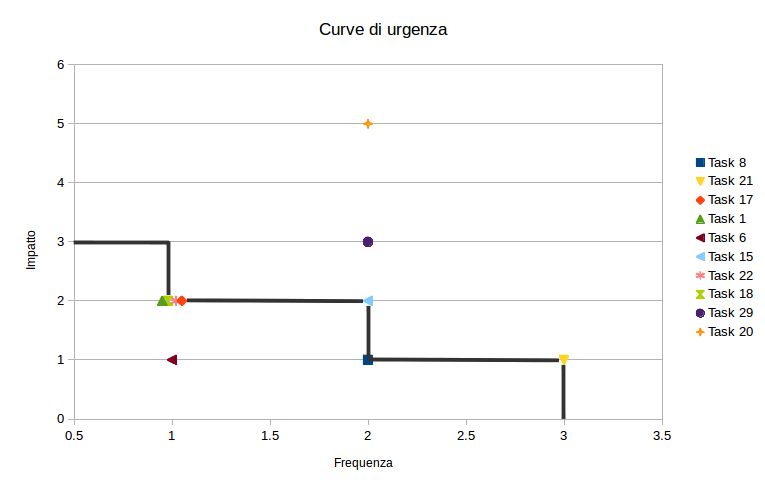
\includegraphics[width=\linewidth]{img/curve-urgenza.png}
\end{figure}

Notiamo subito che i task più urgenti da risolvere sono il task 20 e il
task 29.

\subsection{Miglioramenti}
Dopo aver condotto i test abbiamo apportato delle modifiche al fine di
andare incontro ad alcuni dei problemi riscontrati.\\
È stata data maggiore priorità agli errori che sono risultati urgenti
seocondo le curve di urgenza.

Inanzitutto si è cercato di risolvere il task 20 aggiungendo un pulsante
ben visibilei per la richiesta di aiuto live.\\


\begin{figure}[H]
	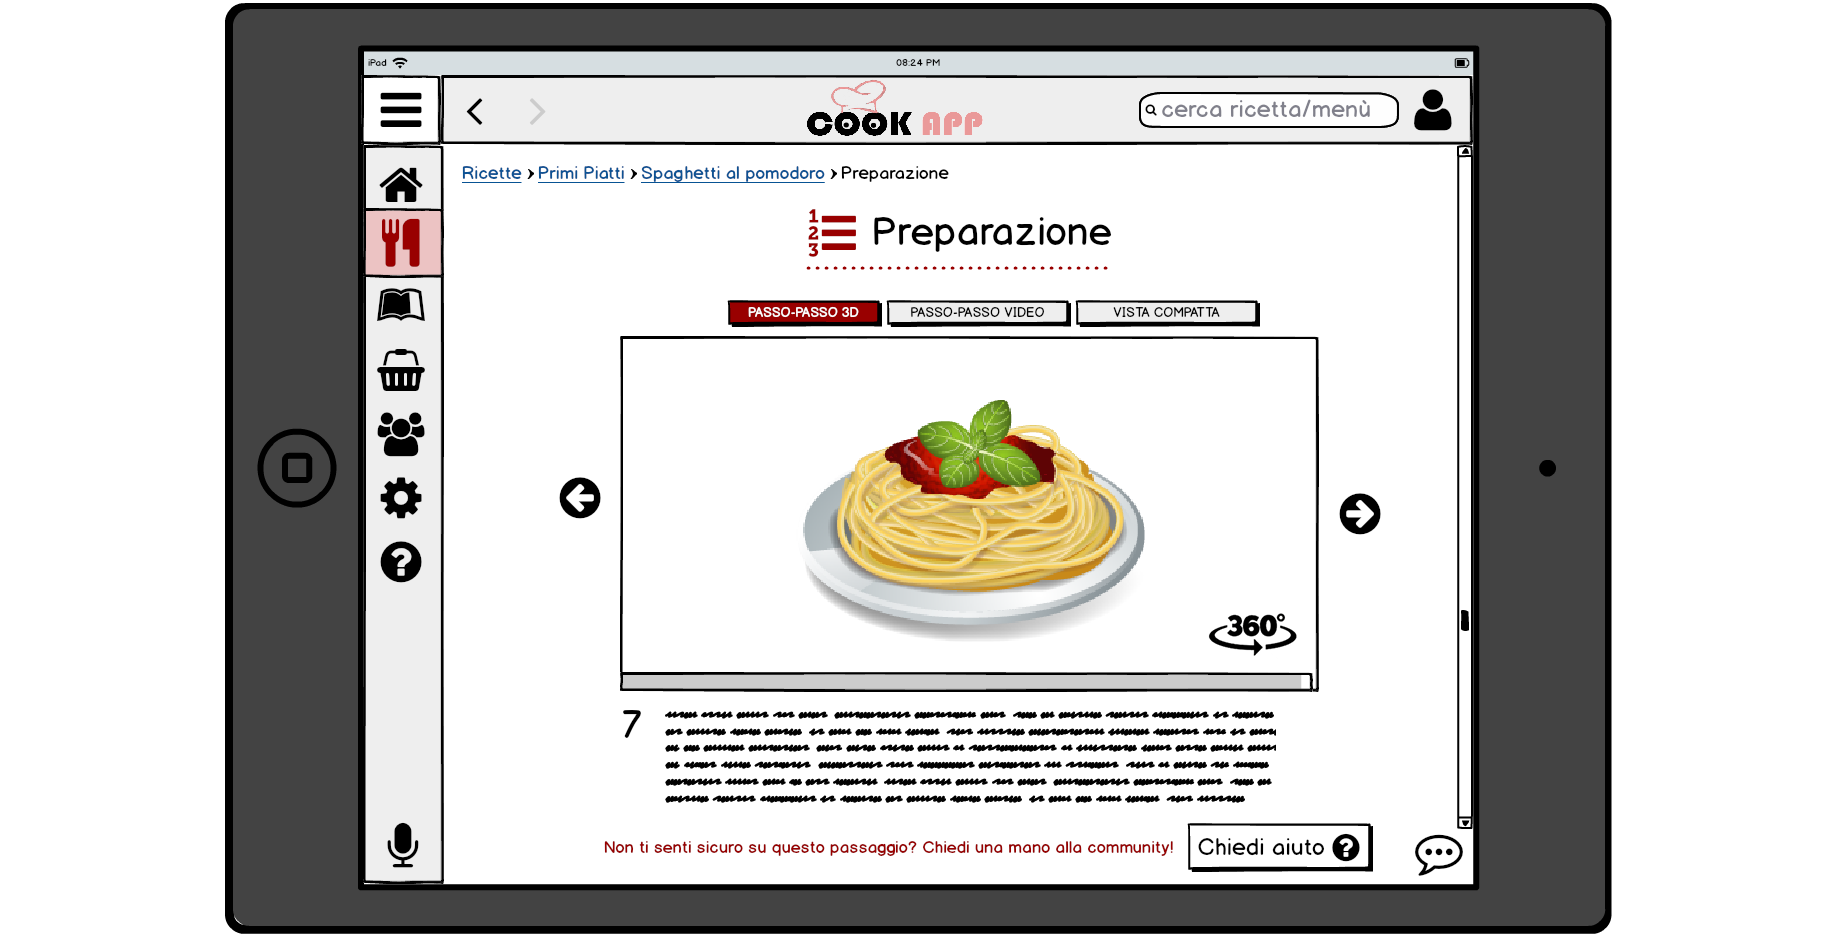
\includegraphics[width=\linewidth]{img/mockup/Ricetta3-fixed.png}
\end{figure}

\begin{figure}[H]
	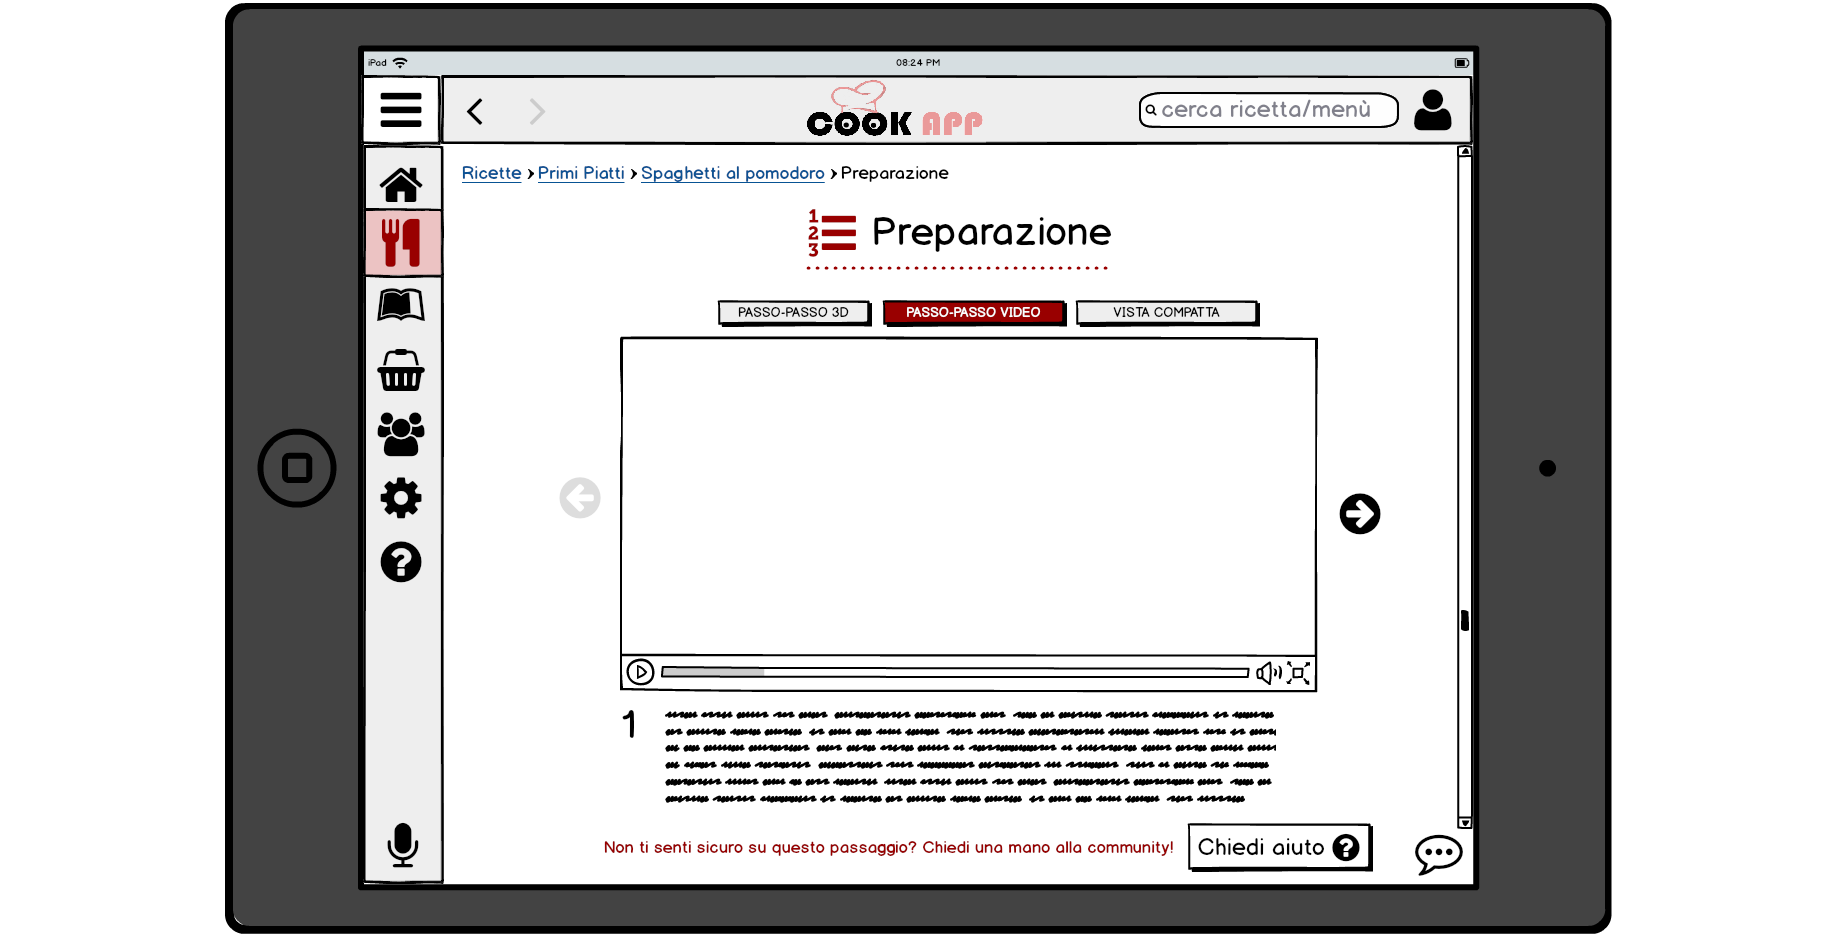
\includegraphics[width=\linewidth]{img/mockup/Ricetta4-fixed.png}
\end{figure}

\begin{figure}[H]
	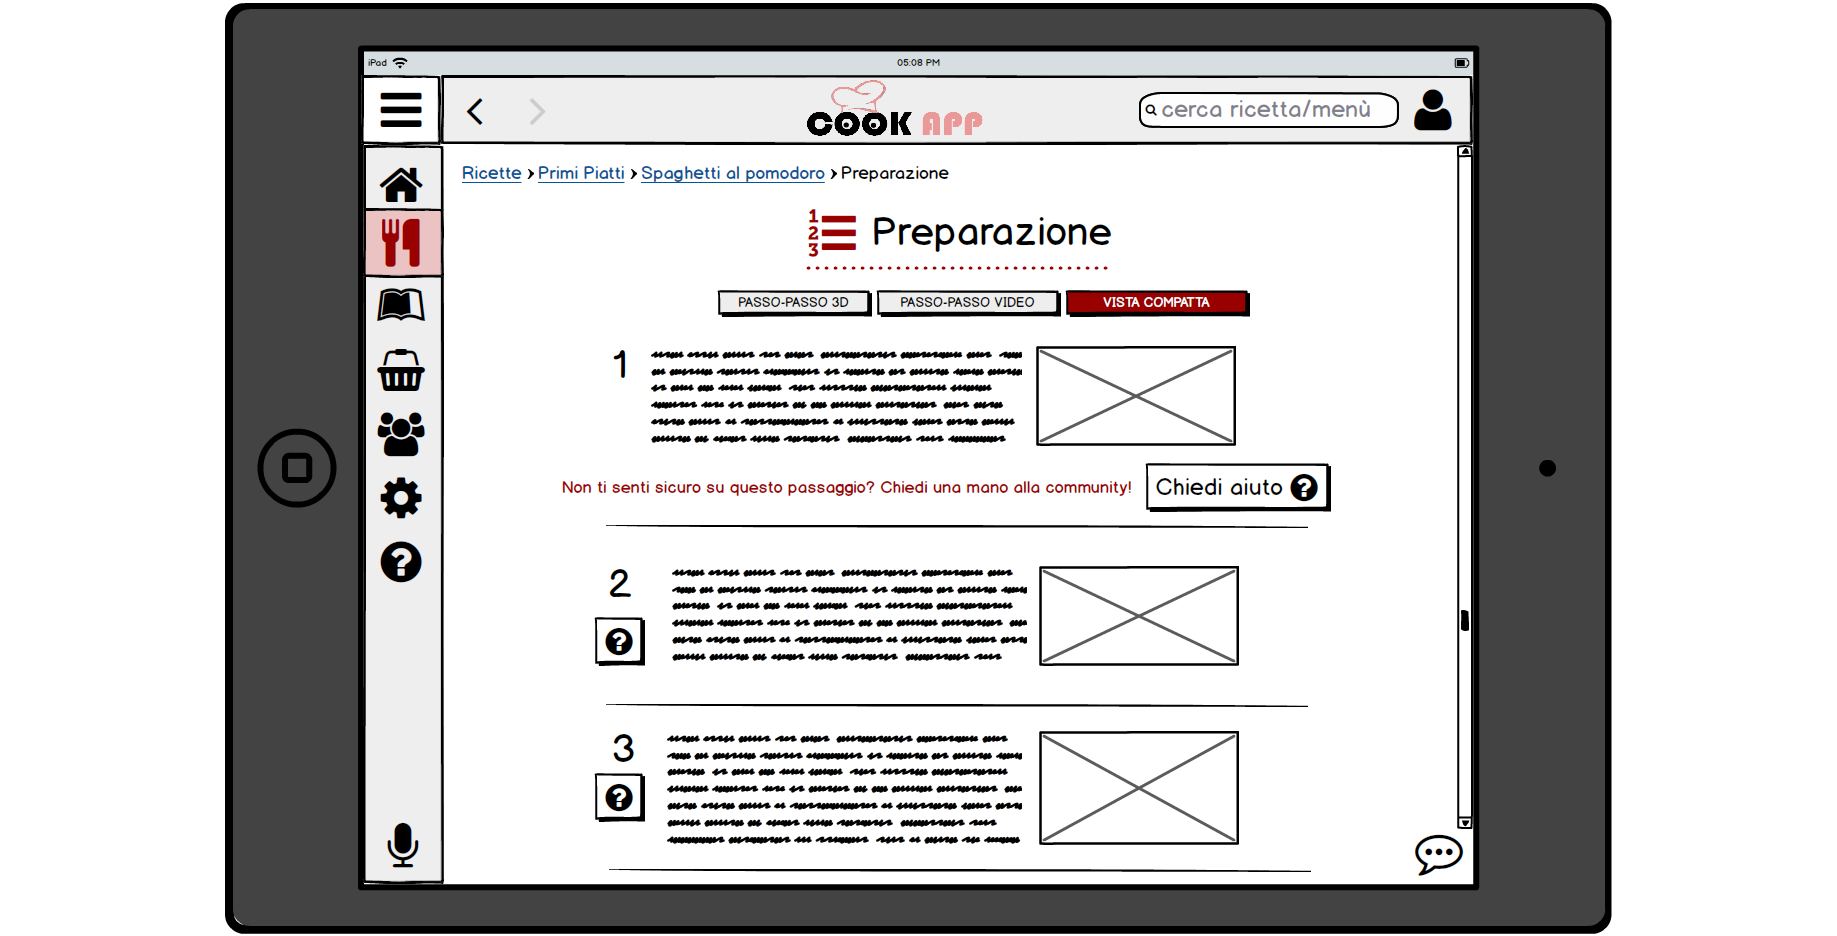
\includegraphics[width=\linewidth]{img/mockup/Ricetta5-fixed.png}
\end{figure}

Durante la realizzazione di questa modifica abbiamo anche
pensato di inserire un pulsante per specificare manualmente qual'è il
problema della fase corrente dopo aver richiesto un aiuto live.

\begin{figure}[H]
	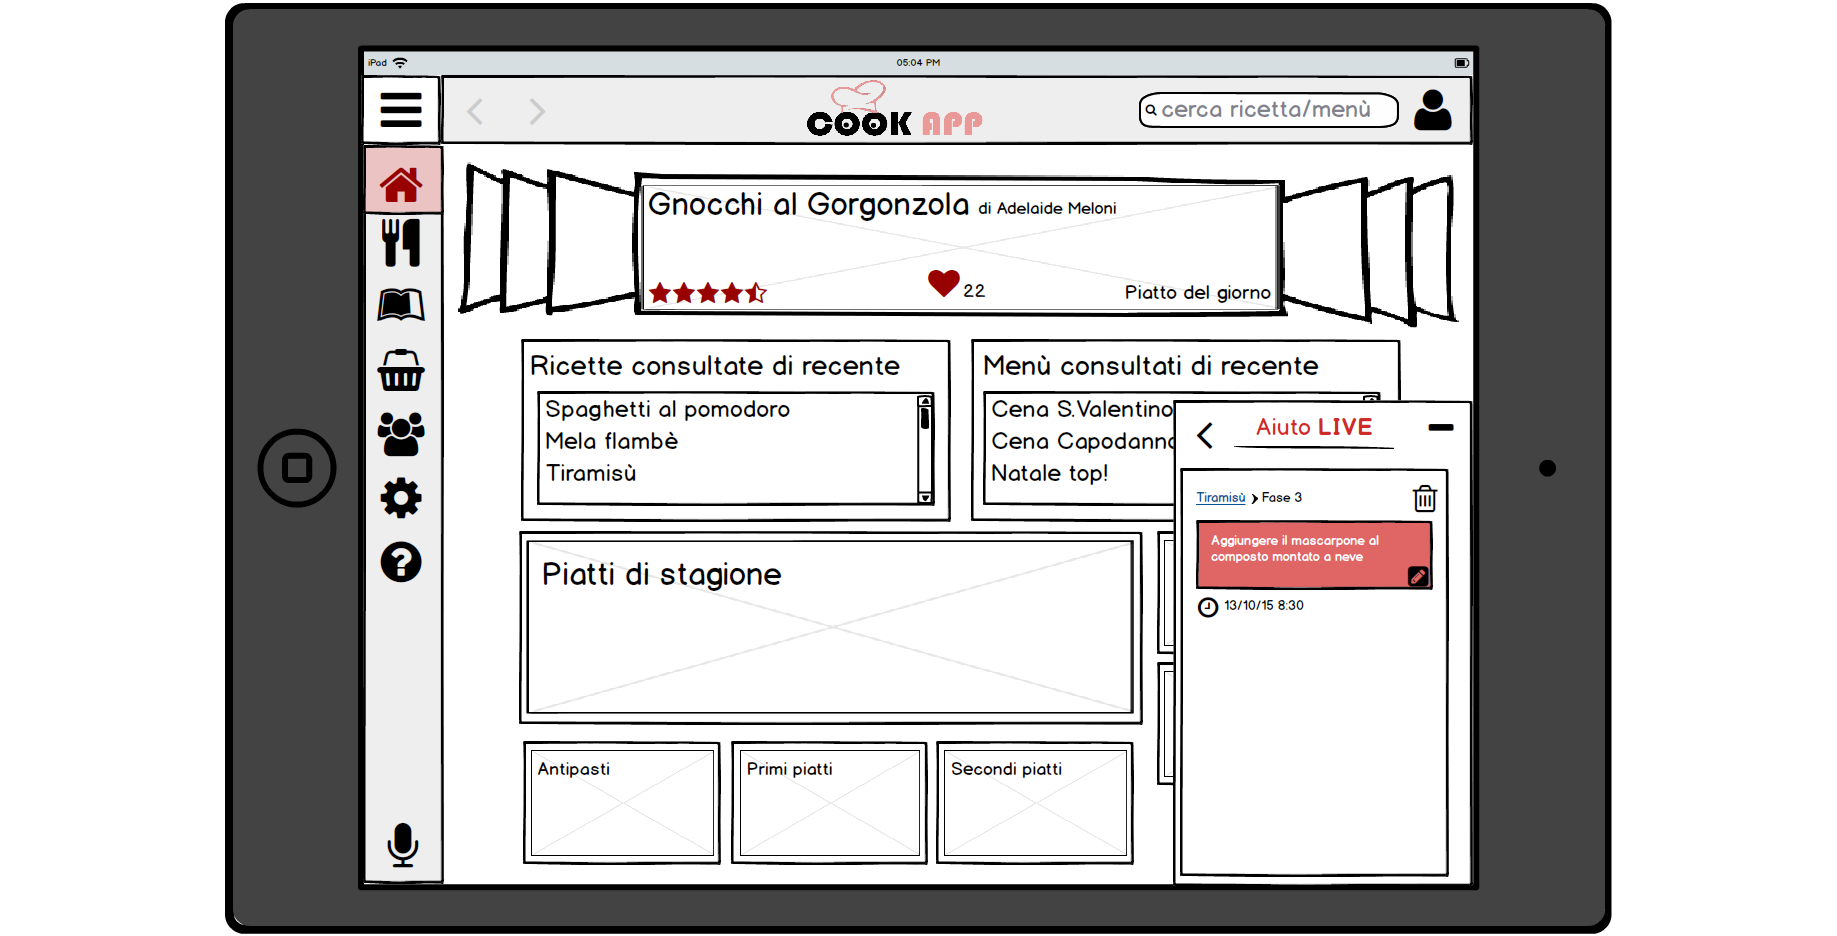
\includegraphics[width=\linewidth]{img/mockup/Live2-fixed.png}
\end{figure}

\begin{figure}[H]
	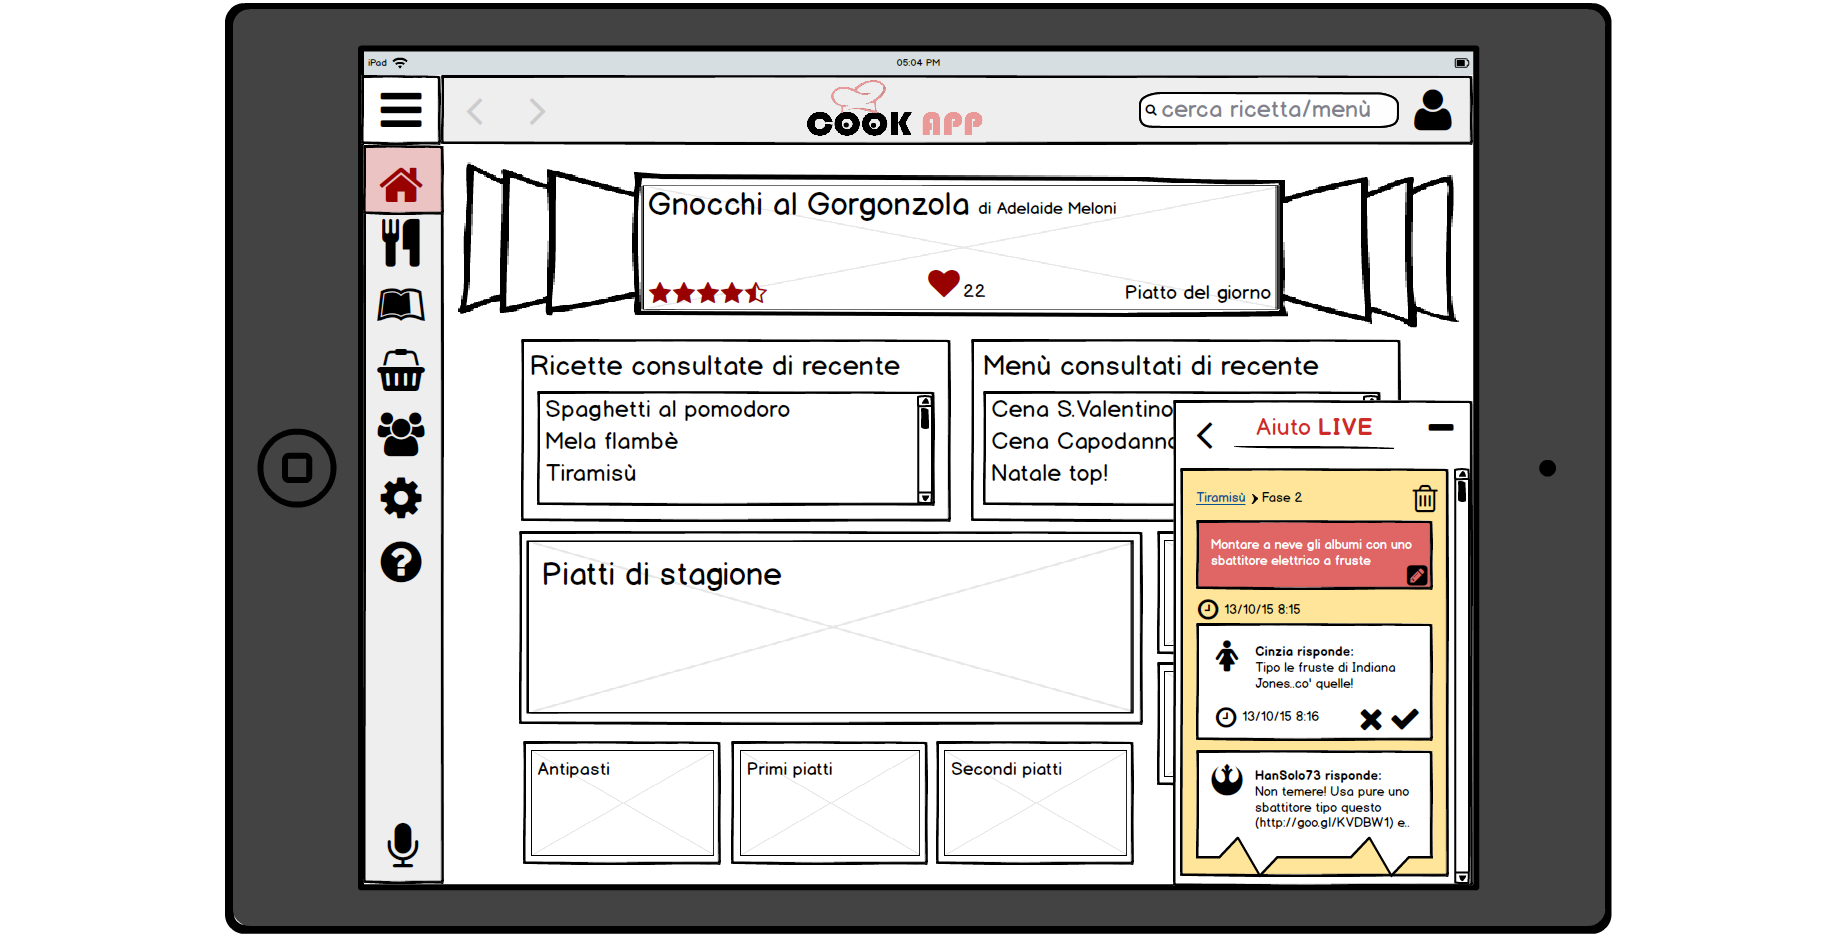
\includegraphics[width=\linewidth]{img/mockup/Live3-fixed.png}
\end{figure}


Successivamente abbiamo anche modificato l'interfaccia per porre rimedio al
problema del task 29, rimuovendo l'icona per annullare le modifiche in
quanto sembrava confondere troppo gli utenti.


\begin{figure}[H]
	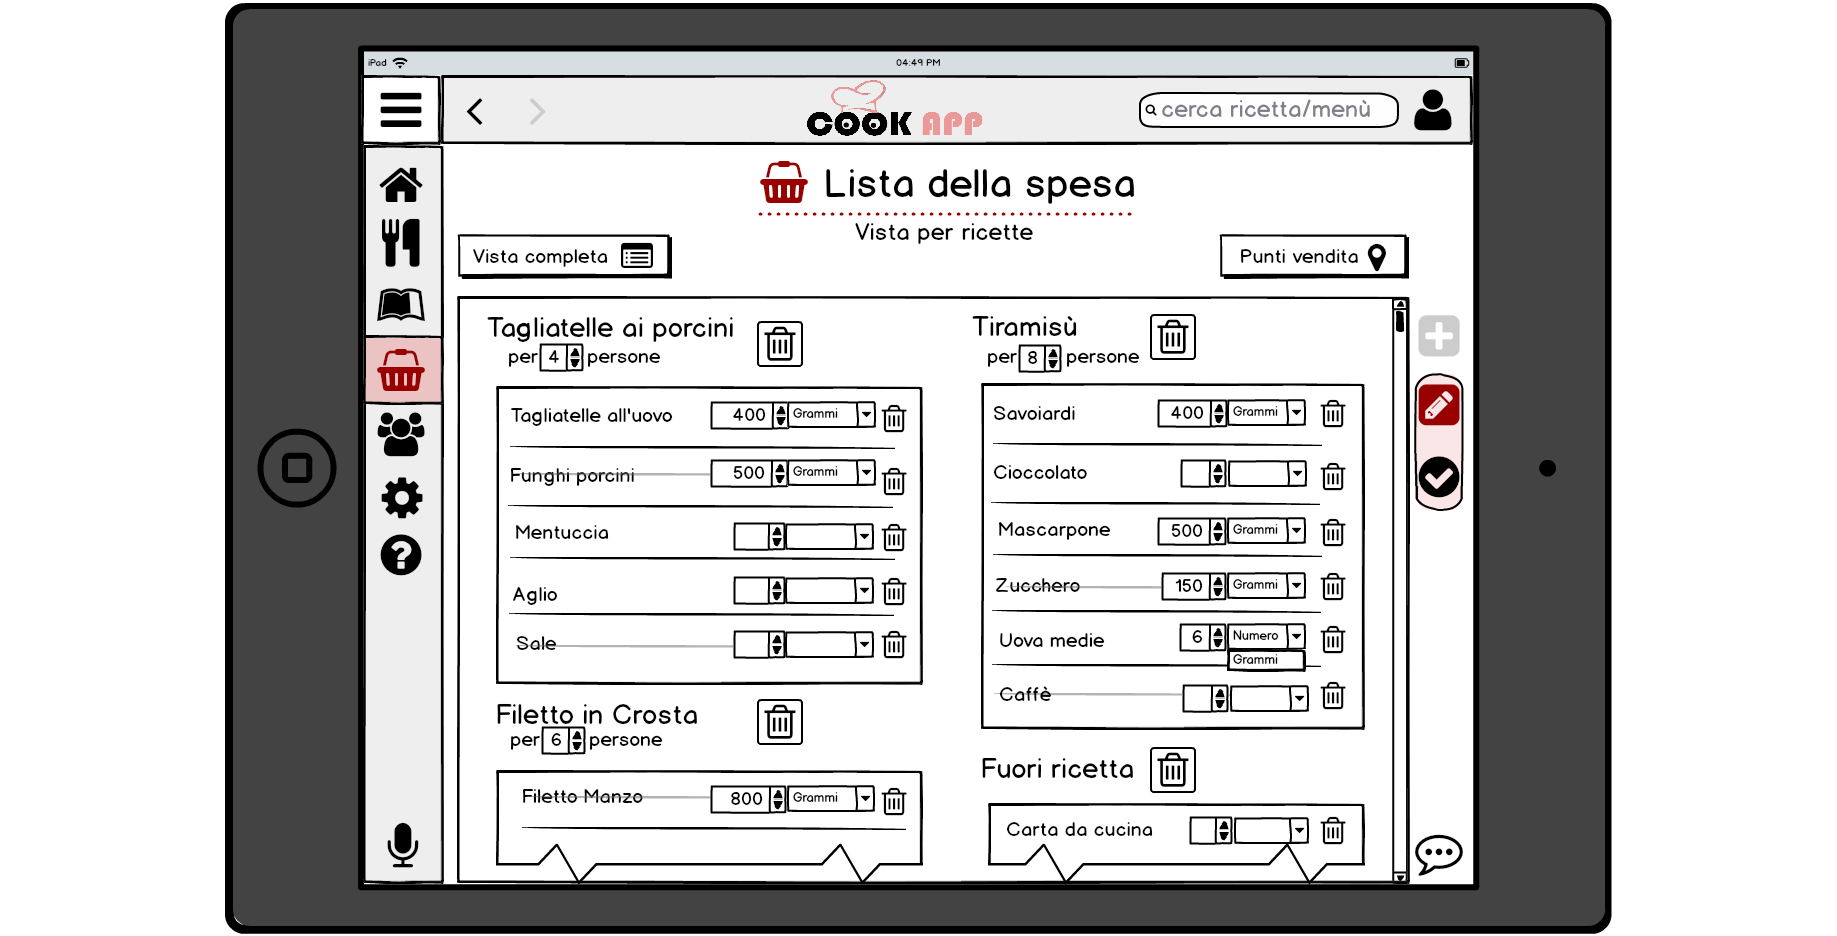
\includegraphics[width=\linewidth]{img/mockup/spesa-edit-fixed.png}
\end{figure}


Infine abbiamo anche risolto facilmente il problema cosmetico 
rilevato dai test del task 8 utilizzando lo stesso colore sia per le
incone del
livello di difficoltà delle ricette che per le icone che ne indicano il
costo delle materie prime.

\begin{figure}[H]
	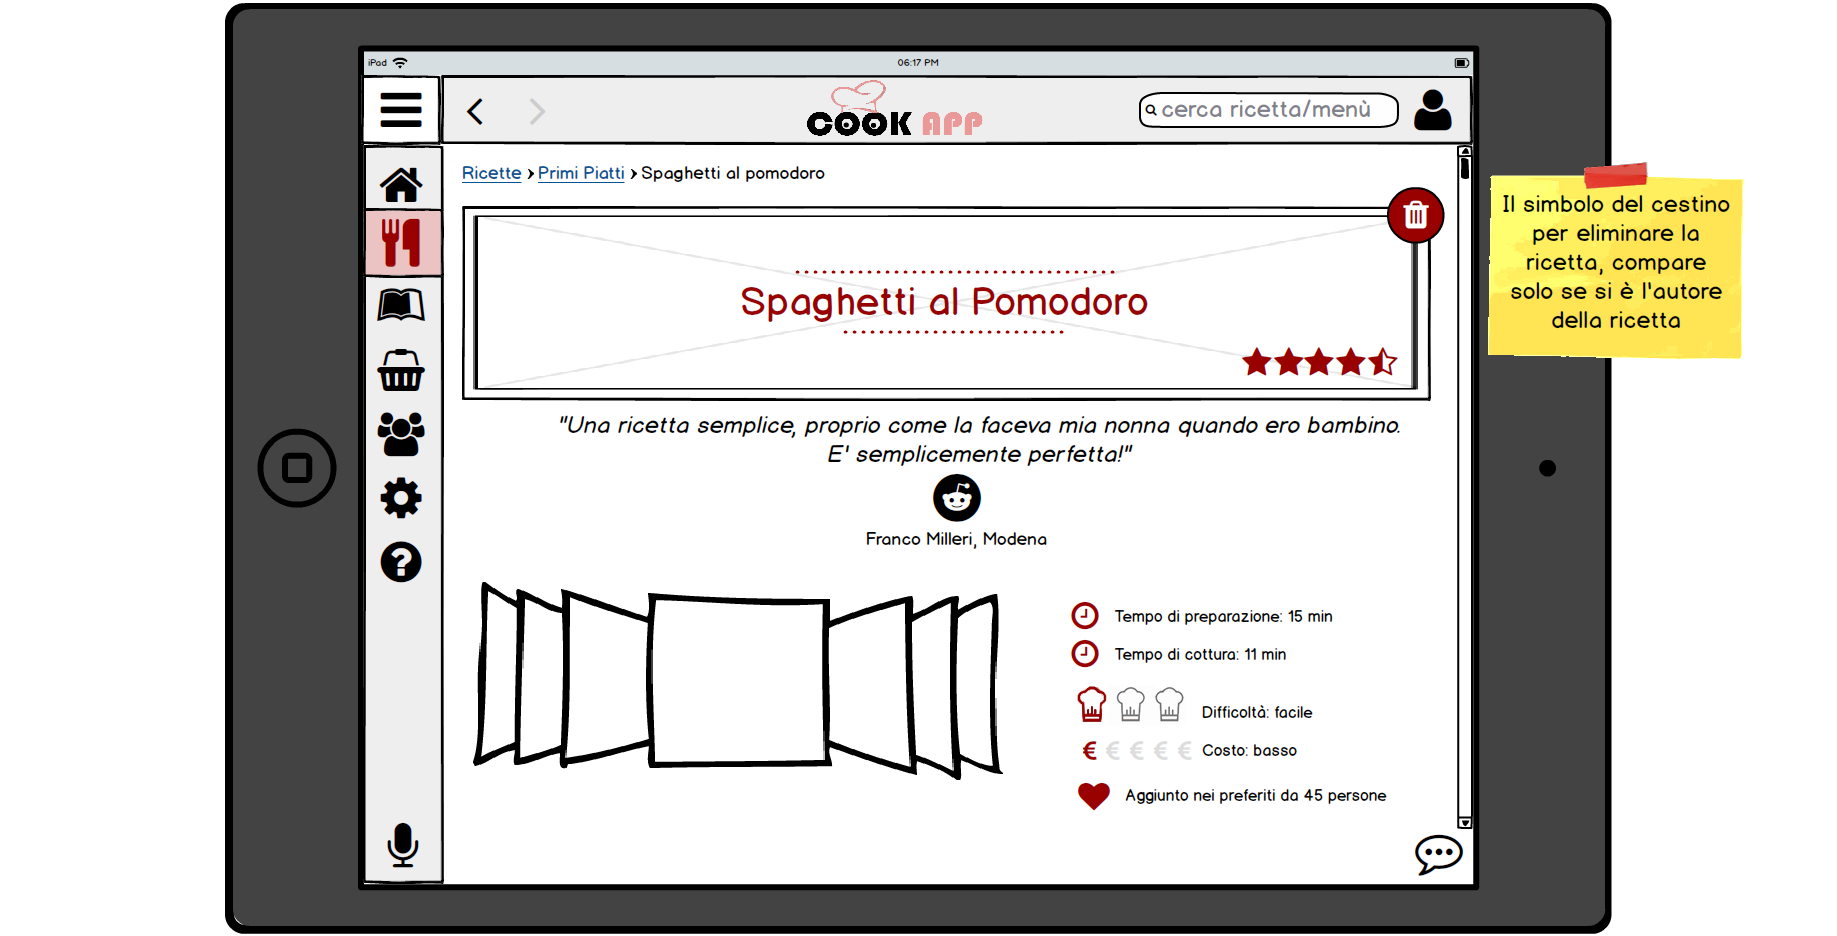
\includegraphics[width=\linewidth]{img/mockup/Ricetta-fixed.png}
\end{figure}
